\section{Introduction}
\label{sec:introduction}

A distributed ledger is a type of distributed database which tolerates nodes with malicious intentions in the system.
And distributed ledger technology (DLT) enables the realization and operation of distributed ledgers,
which allows benign nodes, to agree on an almost immutable record of transactions with Byzantine failure tolerance (BFT) and eventual consistency via a predefined consensus mechanism \cite{Sunyaev2020}.
Blockchain is one of the most well-known DLTs which was first implemented on Bitcoin. It proposed a simple but robust way for transaction data storage without relying on trust of third parties \cite{nakamoto2008peer}.
Blockchain also ensures improved security and anonymity of Bitcoin transactions compared with traditional electronic transactions.
Since the introduction of Bitcoin in 2009, DLT based cryptocurrencies have made a great impact on financial sectors. Later on people also discovered that the usefulness of DLTs is beyond exchange of currencies and
significant adoption of DLTs were made in many other industries for other different services.
Namecoin is the first \texttt{altcoin}\footnote{Altcoin: any cryptocurrencies that are not Bitcoin.} for being the first to create its own blockchain separate from Bitcoin's \cite{kalodner2015empirical}.
And its functionalities are not limited to financial transactions.
The creation of Namecoin was inspired by the idea of BitDNS \cite{merited2010bitdns} and for establishing a decentralized domain name looking up system.


The Internet today is a widespread information infrastructure and its history can date back to 1970s, when \texttt{ARPANET}\footnote{ARPANET: Advanced Research Projects Agency Network.
    The first wide-area packet-switching network with distributed control originally established by United States Department of Defense.} was developed.
For most of the current Internet applications, data is stored in a centralized manner and users don't really own data by themselves. As shown in figure~\ref{fig:traditional_internet},
if users want to do actions like checking their emails or browse the content of a website, they need to connect to the web servers via the Internet with web browsers, then the web servers retrieves the data from the database and then send it back to users.
Usually users' data is hidden behind service providers' application code. This kind of arrangement has been very successful as it is easy to implement. However, it is not ideal since:
\begin{itemize}
    \item Users must use requested web user interface if they want to access their data.
    \item The websites control the rules and access right of the data.
    \item The websites may snoop your data and sell users' information to others.
    \item Illegal use of data by websites' employees for personal purpose.
\end{itemize}

\begin{figure}[h]
    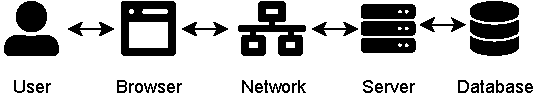
\includegraphics[width=0.45\textwidth,trim={-1cm 0 0.25cm 0},clip]{figs/traditional_internet.pdf}
    \caption{User data arrangement traditional (centralized) Internet application}
    \label{fig:traditional_internet}
\end{figure}

Since the early Internet, hosts in the network were assigned names for more convenient use and memorization by humans. With the growth of the network, it became impossible to store all the hosts in a single table.
And Domain Name System (DNS) invented by Paul Mockapetris of USC/ISI permitted a scalable distributed mechanism for resolving hierarchical host names into Internet addresses \cite{leiner2009brief}.
The coordination and management of DNS Root, IP Addressing, and other Internet protocols are in the charge of \texttt{IANA}\footnote{IANA: Internet Assigned Numbers Authority. Website: \url{https://www.iana.org}} \cite{Postel1994DomainNS}.
These DNS root servers are central nodes of trust and failure, and cyber attack such as \texttt{DDoS}\footnote{DDoS: Distributed Denial-of-service Attack.
    Usually the attack attempts to disrupt the normal traffic of the victim's server by a large amount of requests made by attacker devices.} may leads to the whole system taken down.
It is reported that 13 root servers were under DDoS attack on March 21st, 2002. Fortunately the attack only lasted for one hour and didn't cause severe damage \cite{mcguire2002attack}.
These central points may also be exploited and misleading users into connecting to malicious attack like the incident of Turkish fake site certs \cite{rosenblatt_2013}.


Internet-of-Things (IoT) refers to \textit{"physical or virtual objects which connects to the Internet and has the ability to communicate with human users or other objects"} \cite{6978614}.
These devices such as smart webcam and wearable health monitors are widely used in our daily life.
It is estimated that there will be approximately 30.9 billion active IoT device connections installed worldwide by 2021 \cite{statista_2021}.
Due to heterogeneity and complexity of IoT devices, their security and privacy issues are becoming more and more severe \cite{6978614}.
And with the increasing number of devices connected to the network, load of centralized servers for handling the connection will become much higher.
DLT supported IoT has been created for addressing the challenges like security, data integrity and reliability, and secured P2P sharing. 
It is a new decentralized and distributed solution to IoT services and enables the opportunity for developing new and creative applications and business models in vertical domains, e.g., from healthcare to supply chain, energy industry, and smart manufacturing \cite{Farahani2020TheCO}.


\begin{onehalfspace}
\end{onehalfspace}
\noindent\textbf{Motivation.} Many data management issues like security, integrity, access control has been exposed from centralized data model of traditional Internet. 
When accessing the web services, user data control are maintained by service vendors rather than users themselves.
Domain Name System containing central nodes like DNS root servers are vulnerable to cyber attacks such DDoS. 
Distributed ledger technology such as blockchain can enhance security and data integrity of IoT services. 
However, many of the current DLTs are based on Proof-of-Work (PoW) consensus mechanism \cite{10.1145/2976749.2978341}, which requires very strong computing power and large energy consumption for solving hash computational puzzles.
These mechanisms are not suitable for IoT devices that have poor computational power and strict energy consumption limitation. Transaction fees paid to the miners in the network caused an extra cost for the service. 
DLTs like Bitcoin blockchain are also facing problems like low \texttt{TPS}\footnote{TPS: Transaction Per Second. The approximate average TPS of Bitcoin blockchain is around 5.}, bad scalability, etc.
They are not suitable for IoT service scenarios like sending large amount of micro-transactions in a short period of time. We wish to re-decentralize the current Internet service via distributed ledger technology for better security and data integrity.
We also require the DLT used should be feeless, lightweight, and scalable which can support the use cases of IoT services.


\begin{onehalfspace}
\end{onehalfspace}
\noindent\textbf{Contribution.} We introduce the design and implementation of Vivian, a global naming and storage system secured by IOTA Tangle distributed ledger. 
It is a new decentralized Public Key infrastructure (PKI) system that enables users to register human-readable and unique domain name with binding information. 
By using IOTA Tangle DLT, no central trust points are needed and users can control their own data. 
Peer-to-peer network based on Kademlia DHT and mDNS peer discovery, and Gossip protocol ensures secure data sharing among nodes in the network.
IOTA Tangle is a directed-acyclic-graph (DAG) based distributed ledger which performs better scalability than traditional blockchains. There is no miner involved in the network so no transaction fee is needed.
The whole system is lightweight and enables the possibility of building decentralized IoT applications.